Графиком функции такого вида является справа от OY - подобная параболе ветка, слева  - такая же только идущая вниз. График является симметричным относительно центра координат.

Фигура называется симметричной относительно точки О, если для каждой точки фигуры симметричная ей точка относительно точки О также принадлежит этой фигуре. Точка О называется центром симметрии фигуры.

\begin{figure}[h!]
	\centering
	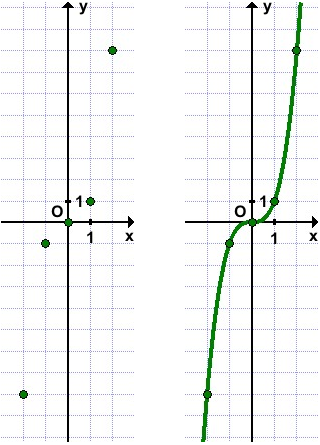
\includegraphics[width=0.5\textwidth]{img/kub.png}
	\caption{Кубическая функция}
\end{figure}

В общем виде: $y = ax^3+bx^2+cx + d$ - поступаем аналогично параболе.

(?) Как строится график функции $y = \sqrt[3]{x}$?